% !TEX TS-program = pdflatex
% !TEX encoding = UTF-8 Unicode
% !TEX root = main.tex
% !TEX spellcheck = en-US
% ****************************************************************************************
% File: main.tex
% Author: Jakob Spindler
% Date: 2024-10-16
% ****************************************************************************************
\documentclass[a4paper,11pt,oneside,final,titlepage,openany,onecolumn]{report}
% input preamble (include additional packages, set options, define macros)
% !TEX TS-program = pdflatex
% !TEX encoding = UTF-8 Unicode
% !TEX root = ../main.tex
% !TEX spellcheck = en-US
% ****************************************************************************************
% File: _preamble.tex
% Author: Jakob Spindler
% Date: 2024-10-16
% ****************************************************************************************
% ****************************************************************************************
% General settings (input encoding, font encoding, font, language)
% ****************************************************************************************
\usepackage[utf8]{inputenc} % character encoding used in input file
\usepackage[T1]{fontenc} % specifies the encoding used in the fonts
\usepackage{lmodern} % provides more support for non-ASCII characters than cm-super
\usepackage{microtype} % improves line-filling when using PDFLaTeX
\usepackage[ngerman,english]{babel} %  last language is considered the main one
\renewcommand{\familydefault}{\sfdefault} % select a sans serif font family 

% \pdfsuppresswarningpagegroup=1 % suppress warning when including PDFs with page groups

% ****************************************************************************************
% Basic macros for thesis
% ****************************************************************************************
\newcommand{\authorName}{Jakob Spindler}
\newcommand{\authorContact}{sj0458@mci4me.at}

\newcommand{\department}{Department of Technology \& Life Sciences}
\newcommand{\docTitle}{Discrete PID Controller Design for a Buck Converter}
\newcommand{\docType}{Report}
\newcommand{\studyProgram}{Master's program Mechatronics \& Smart Technologies}
\newcommand{\degree}{Master of Science in Engineering}
\newcommand{\studyYear}{MA-MECH-23-VZ}
\newcommand{\supervisorName}{Thomas Gadner}
\newcommand{\supervisorContact}{}
\newcommand{\assesorName}{Dr. Georg Saxl}
\newcommand{\assesorContact}{georg.saxl@mci.edu}
\newcommand{\university}{Management Center Innsbruck}
\newcommand{\matnr}{11941482}


\newcommand{\authorAName}{Liam Nolan}
\newcommand{\authorAContact}{nl6496@mci4me.at}
\newcommand{\authorBName}{Johannes Schmid}
\newcommand{\authorBContact}{sj0751@mci4me.at}
\newcommand{\authorCName}{Jakob Spindler}
%\newcommand{\authorCContact}{sj0458@mci4me.at}
\newcommand{\courseName}{WS 2024 Transient Simulation }
\newcommand{\courseCode}{MECH-M-3-SVE-TSI-ILV
}
%\newcommand{\department}{Department of Technology \& Life Sciences}
%\newcommand{\docTitle}{Optimization Study of a flow heater}
%\newcommand{\docType}{Report}
%\newcommand{\studyProgram}{Master's program Mechatronics \& Smart Technologies}
%\newcommand{\studyYear}{MA-MECH-23-VZ}
\newcommand{\lecturerName}{Manuel Berger, PhD}
\newcommand{\lecturerContact}{manuel.berger@mci.edu}
%\newcommand{\university}{Management Center Innsbruck}
% Definition of BibTeX macro used in IEEEexample
\newcommand{\BibTeX}{BibTeX}

% ****************************************************************************************
% Drawing and plotting, scientific packages, 
% ****************************************************************************************
% For use of subfigure environment
\usepackage{subcaption}

% For use of cmidrule in table environment
\usepackage{booktabs}

\usepackage{makecell}

% Handling of images
\usepackage{graphicx}
\graphicspath{{./img/}}

% Colour support
\usepackage[table]{xcolor}

% Handling of MATLAB code
%\usepackage{mcode}

% Tabulars with adjustable-width columns
\usepackage{tabularx}
\usepackage{multirow}

% Sketching and importing MATLAB plots
\usepackage{pgfplots}
\usepackage{grffile}
\pgfplotsset{compat=newest}
\usetikzlibrary{plotmarks}
\usetikzlibrary{arrows.meta}
\usetikzlibrary{patterns}
\usepgfplotslibrary{patchplots}
\pgfplotsset{plot coordinates/math parser=false}
\newlength\figureheight
\newlength\figurewidth

% Typesetting electrical networks
\usepackage{circuitikz}

% scientific packages
\usepackage{amsmath}
\usepackage{amsfonts}
\usepackage{xfrac}
\usepackage{siunitx}
\AtBeginDocument{\sisetup{
		mode=match,
		unit-font-command = \mathrm,
		reset-text-family=false,
		reset-text-series=false,
		reset-text-shape=false,
		exponent-product=\cdot
	}}
\DeclareSIUnit\unity{1} % can be used for dimensionless quantities
\DeclareSIUnit\sample{Sa}
% ****************************************************************************************
% Referencing and citing
% ****************************************************************************************
% Caption settings
\usepackage[
	format=plain, % typeset as normal paragraph
	labelformat=simple, % typeset label as name and number
	labelsep=period, % caption label and text separated by period and space
	textformat=simple, % caption text typeset as is
	justification=justified, % typset caption as normal paragraph
	singlelinecheck=true, % automatically center short captions
	font=small,
	labelfont=bf, % set bold font for label
	width=.75\textwidth % set fixed width for caption
]{caption}
\captionsetup[table]{position=top}
\captionsetup[figure]{position=bottom}

% Hypertext marks (should be loaded last but before geometry)
\usepackage[hyperindex]{hyperref}
% Extension options
\hypersetup{
	colorlinks, % colours the text of links and anchors (instead of borders)
	linkcolor={blue!65!black},
	citecolor={blue!65!black},
	urlcolor={blue!65!black}
}
% PDF display and information options
\hypersetup{
	pdftitle={\docTitle},
	pdfsubject={\docType},
	pdfauthor={\authorName},
	pdfkeywords={},
	pdfcreator={pdflatex},
	pdfproducer={LaTeX with hyperref}
}

% formatting of cross-references
\usepackage[capitalise]{cleveref}
\crefformat{equation}{(#2#1#3)}
\Crefformat{equation}{Equation~(#2#1#3)}

%matlab prettifier
\usepackage{matlab-prettifier}

% ****************************************************************************************
% Bibliography settings
% ****************************************************************************************
% template from https://www.ieee.org/conferences/publishing/templates.html
\usepackage[
	backend=biber,
	style=numeric-comp, % numeric style with compact multiple citations i.e. [1-5] and not [1,2,3,4,5]
	natbib=true,
	sorting=none
]{biblatex}
%\addbibresource{zotero.bib}
\addbibresource{bib.bib}

% ****************************************************************************************
% Glossary (acronyms, list of symbols) settings
% ****************************************************************************************
\usepackage[acronym,nomain,nonumberlist,nopostdot,sort=def,toc]{glossaries}
\renewcommand*{\glstextformat}[1]{\textcolor{black}{#1}} % make links appear black
\newglossary[slg]{symbolslist}{syi}{syg}{List of Symbols} % define custom glossary
\glsaddkey% define custom key
	{unit}% key
	{\glsentrytext{\glslabel}}% default value
	{\glsentryunit}% command analogous to \glsentrytext
	{\GLsentryunit}% command analogous to \Glsentrytext
	{\glsunit}% command analogous to \glstext
	{\Glsunit}% command analogous to \Glstext
	{\GLSunit}% command analogous to \GLStext
\glssetnoexpandfield{unit}
\makeglossaries % create makeindex files

\newglossarystyle{symbolsliststyle}{%
	\setglossarystyle{long3col}% style based on long3col
	\renewenvironment{theglossary}{%
		\begin{longtable}{lp{\glsdescwidth}>{\arraybackslash}p{2cm}}}%
		{\end{longtable}}%
	\renewcommand*{\glossaryheader}{% change the table header
		\bfseries Symbol & \bfseries Description & \bfseries Unit\\\hline%
		\endhead}%
	\renewcommand*{\glossentry}[2]{% change the displayed items
		\glstarget{##1}{\glossentryname{##1}}% name
		& \glossentrydesc{##1}% description
		& $\glsentryunit{##1}$% unit
		\tabularnewline
	}%
}

% ****************************************************************************************
% Page layout and headers
% ****************************************************************************************
% Specify page layout (paper name and orientation specified in document class options)
\usepackage[
	includeheadfoot, % includes the head of the page into total body
	ignoremp, % disregards marginal notes in determining the horizontal margins
	nomarginpar, % shrinks spaces for marginal notes to 0pt
	hmargin=1.5in, % left and right margin
	vmargin=1in, % top and bottom margin
	headheight=14pt %  height of header
]{geometry}

\usepackage{parskip} % helps in implementing paragraph layouts

% Header and footer settings
\usepackage{fancyhdr}
\pagestyle{fancy} % set page style to 'fancy'
\renewcommand{\chaptermark}[1]{\markboth{\thechapter.\ #1}{}}
% \renewcommand{\sectionmark}[1]{\markright{\thesection.\ #1}}
\fancyhf{} % clear all header and footer fields
\fancyhead[L]{\leftmark} % set left header location (chapter)
% \fancyhead[R]{\rightmark} % set right header location (section)
\fancyfoot[C]{\thepage} % set center footer location (page count)

% ****************************************************************************************
% Packages for testing purposes (can be deleted)
% ****************************************************************************************
\usepackage{lipsum}
\usepackage{blindtext}
\usepackage{todonotes}
%\usepackage{superscript}

% EOF
\loadglsentries{./tex/_/_defns.tex}
\makeglossaries
\begin{document}
	\pagenumbering{alph}
	% !TEX TS-program = pdflatex
% !TEX encoding = UTF-8 Unicode
% !TEX root = ../main.tex
% !TEX spellcheck = en-US
% ****************************************************************************************
% File: titlepage.tex
% Author: Jakob Spindler
% Date: 2024-10-16
% ****************************************************************************************

\thispagestyle{empty}
\pdfbookmark[0]{Title page}{titlepage} % sets a PDF bookmark
\thispdfpagelabel{} %  set page number shown in the tool bar of a PDF viewer
\begin{center}
	\textbf{\Huge \university}\par
	\vspace{8ex}\par
	\textbf{\LARGE \department}\par
	\vspace{4ex}\par
	\textbf{\Large \studyProgram}\par
	\vspace{4ex}\par
	
\includegraphics[scale = 0.75]{MCI_Logo.pdf}\par
	\vspace{4ex}\par
	\textbf{\LARGE \docType}\par
	\vspace{2ex}\par
	\textbf{composed as part of the course\\[0.5ex] \courseName{} (\courseCode)}\par
	\vspace{4ex}\par
	\textbf{about}\par
	\vspace{4ex}\par
	\textbf{\LARGE \docTitle}\par
	\vspace{4ex}\par
	\textbf{from}\par
	\vspace{4ex}\par
	\textbf{\Large \href{\authorContact}{\authorName}}
\end{center}
\vspace{4ex}
\begin{tabular}{ll}
	Study program & \studyProgram\\[0.5ex]
	Year & \studyYear\\[0.5ex]
	Course & \courseName{} (\courseCode)\\[0.5ex]
	Name of supervisor & \href{\lecturerContact}{\supervisorName}\\[0.5ex]
	Submission deadline & January 27, 2024
\end{tabular}
\vfill
\begin{center}
	\today
\end{center}
%EOF
	\pagenumbering{Roman}
	\pdfbookmark[0]{\contentsname}{toc} % sets a PDF bookmark
 
    \tableofcontents
	\newcounter{romanpagecount}
	\setcounter{romanpagecount}{\value{page}}
	\clearpage
	\pagenumbering{arabic}

	% add content here
    
    

	% !TEX TS-program = pdflatex
% !TEX encoding = UTF-8 Unicode
% !TEX root = ../main.tex
% !TEX spellcheck = en-US
% ****************************************************************************************
% File: introduction.tex
% Author: Jakob Spindler
% Date: 2024-10-16
% ****************************************************************************************
\chapter{Introduction}
\label{chapter:introduction}

A discrete \gls{acr:pid} controller for a \qty{12}{\volt} to \qty{5}{\volt} Buck-Converter is to be designed and tested using PLECS \autocite{PLECSPlexim}.

The self-imposed charcteristics of the buck converter and the chosen passive components according to \autocite{BuckConverter} are given in \autoref{tab:converter_characteristics} and \autoref{tab:components} respectively.

\begin{table}[htbp]
    \centering
    \begin{minipage}{0.45\textwidth}
        \centering
        \begin{tabular}{c|c}
            Parameter & Value \\ \hline
            $V_{\text{in,nominal}}$ & \qty{12}{\volt} \\ 
            $V_{\text{in,min}}$ & \qty{8}{\volt} \\
            $V_{\text{in,max}}$ & \qty{16}{\volt} \\  
            $V_{\text{out}}$ & \qty{5}{\volt} \\ 
            $I_{\text{out}}$ & \qty{1}{\ampere} \\
            $\Delta I_{\text{L}}$ at $V_{\text{in,max}}$ & \qty{400}{\milli\ampere} \\
            $f_{\text{sw}}$ & \qty{50}{\kilo\hertz}
        \end{tabular}
        \caption{Buck-Converter Characteristics}
        \label{tab:converter_characteristics}
    \end{minipage}\hfill
    \begin{minipage}{0.45\textwidth}
        \centering
        \begin{tabular}{c|c}
            Component & Value \\ \hline
            $L$ & \qty{200}{\micro\henry} \\ 
            $C$ & \qty{50}{\micro\farad} \\ 
            $R$ & \qty{5}{\ohm} \\ 
             \\
        \end{tabular}
        \caption{Passive components \\ of the Buck-Converter}
        \label{tab:components}
    \end{minipage}
\end{table}

A continous controller can be designed according to \autocite{samosirSimpleFormulaDesigning2023} -- for simplicity, the parameters were kept the same for the discrete controller

\begin{table}[htbp]
    \centering
    \begin{tabular}{c|c}
        Parameter & Value \\ \hline
        $K_D$ & $50 LC$ \\ 
        $K_P$ & $50 \frac{L}{R}$ \\ 
        $K_I$ & $50$ \\ 
    \end{tabular}
    \caption{PID Controller Parameters}
    \label{tab:pid_parameters}
\end{table}


% EOF
	% !TEX TS-program = pdflatex
% !TEX encoding = UTF-8 Unicode
% !TEX root = ../main.tex
% !TEX spellcheck = en-US
% ****************************************************************************************
% File: methods.tex
% Author: Jakob Spindler
% Date: 2024-10-16
% ****************************************************************************************
\chapter{Methods}
\label{chapter:methods}

\section{Controller Design}
\label{section:controller_design}

The PLECS model of the converter includes the following:
\begin{itemize}
    \item a PID controlled duty cycle
    \item a noise source for the input voltage
    \item a variable load
\end{itemize}

all of which can be selected to be active or inactive as can be seen in \autoref{fig:PLECS_model} and \autoref{fig:PLECS_subsystems}.

\begin{figure}[htbp]
    \centering
    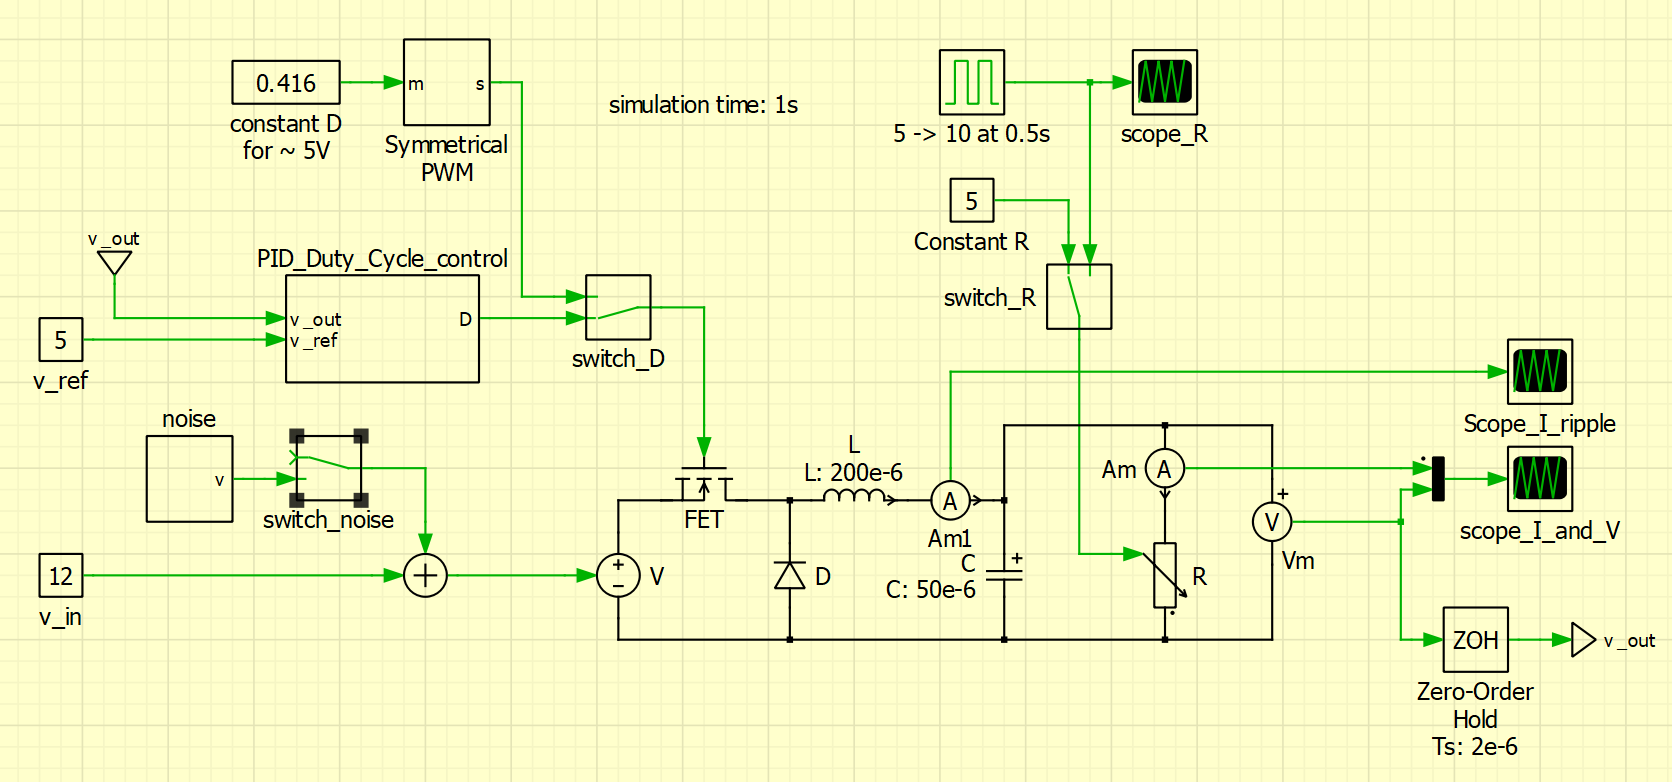
\includegraphics[width=0.95\textwidth]{img/PLECS_model_full_view.png}
    \caption{PLECS model of the Buck-Converter}
    \label{fig:PLECS_model}
\end{figure}

\begin{figure}[htbp]
    \centering
    \begin{subfigure}[b]{0.55\textwidth}
        \centering
        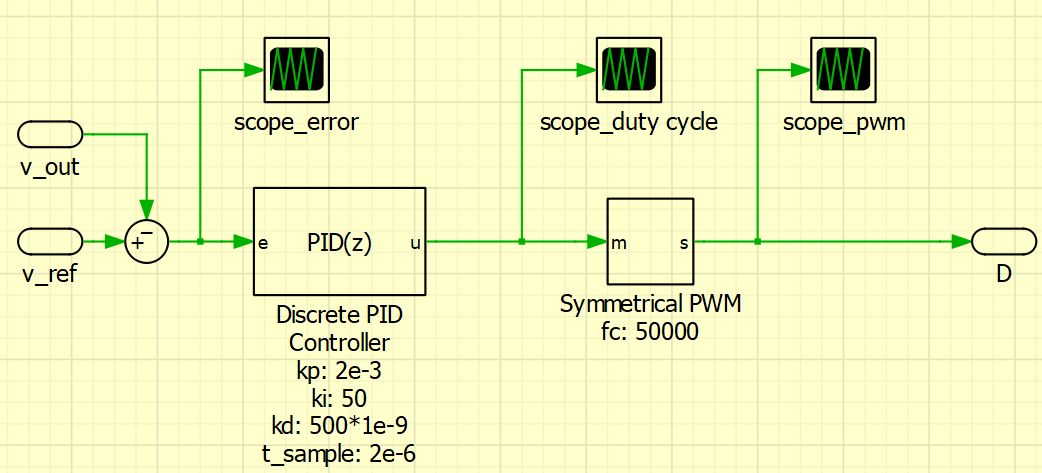
\includegraphics[width=\textwidth]{img/PLECS_PID_Duty_Cycle_control.png}
        \caption{PLECS model of the PID\_Duty\_Cycle\_control subsystem}
        \label{fig:PLECS_PID}
    \end{subfigure}
    \hfill
    \begin{subfigure}[b]{0.40\textwidth}
        \centering
        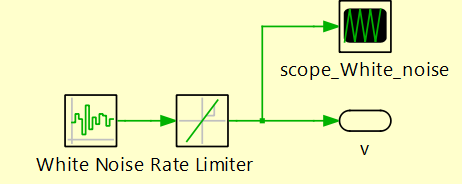
\includegraphics[width=\textwidth]{img/PLECS_noise.png}
        \caption{PLECS model of the noise subsystem}
        \label{fig:PLECS_noise}
    \end{subfigure}
    \caption{PLECS model subsystems}
    \label{fig:PLECS_subsystems}
\end{figure}

\begin{figure}[htbp]
    \centering
    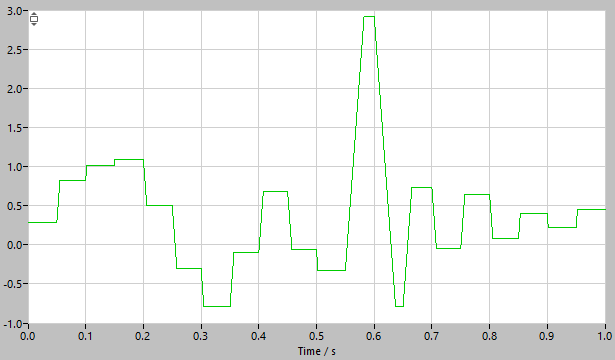
\includegraphics[width=0.8\textwidth]{img/noise.png}
    \caption{White noise with a standard deviation of \qty{1}{\volt} and a sample time of \qty{50}{\milli\second}}
    \label{fig:noise}
\end{figure}

The control of the converter was tested under the following conditions and compared to the behaviour of the converter with a fixed duty cycle:
\begin{itemize}
    \item noise on the input voltage (white noise with a standard deviation of \qty{1}{\volt} and a sample time of \qty{50}{\milli\second} as seen in \autoref{fig:noise})
    \item a load step from \qty{5}{\ohm} to \qty{10}{\ohm} at \qty{0.5}{\second}
    \item startup behaviour
\end{itemize}

\section{Hardware-in-the-Loop (HIL) Setup}
\label{section:hil_setup}

As a next step, the controller-converter system shown in \autoref{section:controller_design} is split into two distinct discrete subsystems that can be used for code generation for the respective hardware and each form the controller and converter respectively. The blocks are connected using real-time interface blocks, like the \textit{Analog In (triggered)} and \textit{PWM} blocks for the Controller and the \textit{Analog Out1} and \textit{PWM Capture1} blocks for the Converter. The generic HIL setup is shown in \autoref{fig:HIL_setup}. The subsystems are then connected into a closed control loop with a scope block to monitor the output of the converter.

\begin{figure}[htbp]
    \centering
    % Top figure
    \begin{subfigure}[b]{0.9\textwidth}
        \centering
        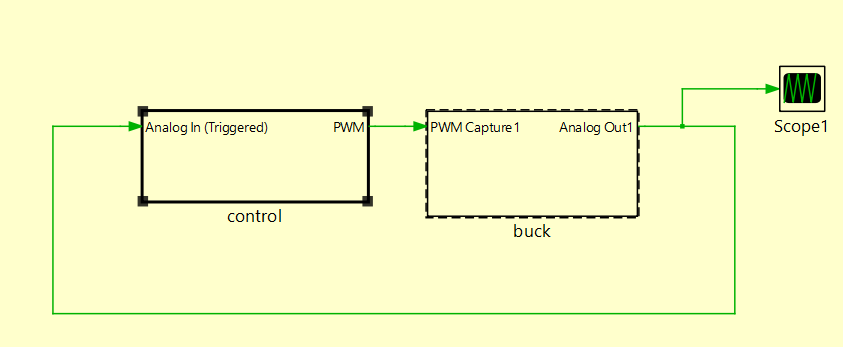
\includegraphics[width=\textwidth]{img/HIL/generic_setup.png}
        \caption{PLECS Model of the generic HIL setup}
        \label{fig:plecs_model_generic_hil}
    \end{subfigure}

    % Bottom row figures
    \begin{subfigure}[b]{0.49\textwidth}
        \centering
        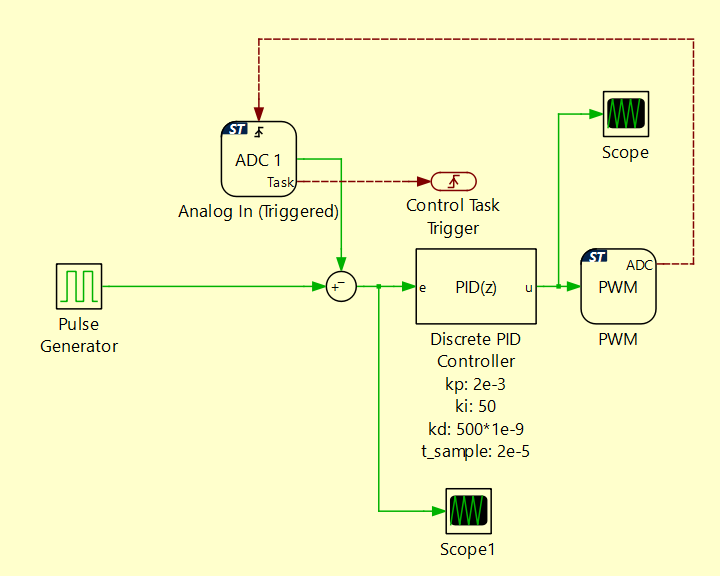
\includegraphics[width=\textwidth]{img/HIL/generic_control.png}
        \caption{Controller Subsystem}
        \label{fig:generic_controller}
    \end{subfigure}
    \hfill
    \begin{subfigure}[b]{0.49\textwidth}
        \centering
        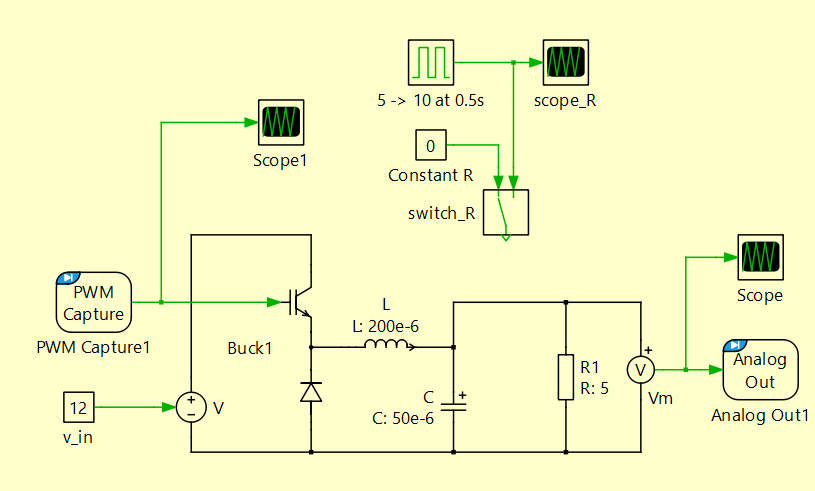
\includegraphics[width=\textwidth]{img/HIL/generic_buck.png}
        \caption{Buck Converter Subsystem}
        \label{fig:generic_buck}
    \end{subfigure}

    \caption{PLECS Generic HIL Setup and Subsystems}
    \label{fig:HIL_setup}
\end{figure}

\subsection{Verification of the Sampling Frequencies}
\label{subsection:sampling_frequencies}

Before actual hardware implementation, it is advisable to verify that the whole system still operates as inteded with descretization parameters for the subsystems set.
As a rule of thumb, the sample frequency of the controller may equal the switching frequency of the converter, while the sample frequency of the converter may be set to a multiple of the switching frequency, ideally 10 to 20 times the switching frequency.

This verification can easily be done withoput hardware by setting the desired sampling frequencies and then generating code for the subsystems with a generic target -- thus enabling code execution on the local machine. By inspecting the output of the converter, a statement can be made about the correct operation of the system.

For simplicity reasons, a reference-voltage-pulse of \qty{10}{\hertz} with a duty cycle of \qty{50}{\percent} and amplitudes of \qty{5}{\volt} and \qty{10}{\volt} was used as the input signal for the controller.
The sampling frequencies were chosen as
\begin{itemize}
    \item $f_{sw}$ for the controller
    \item $10f_{sw}$ for the buck converter
\end{itemize}
The output of the converter is shown in \autoref{fig:verification}.
\begin{figure}[htbp]
    \centering
        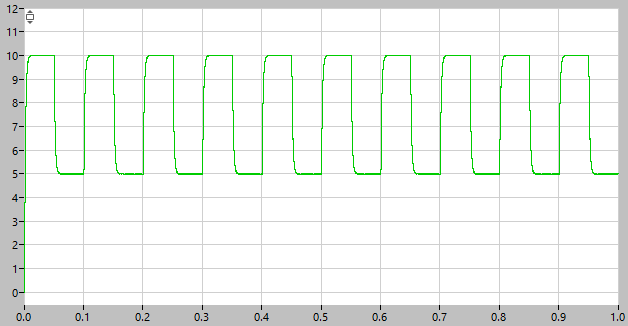
\includegraphics[width=0.8\textwidth]{img/HIL/generic_v_out.png}
    \caption{Buck converter output voltage -- Verification of the HIL setup with local code execution}
    \label{fig:verification}
\end{figure}

\subsection{Hardware Implementation}
\label{subsection:hardware_implementation}
With the verification of the sampling frequencies, the next step is to generate code for the respective hardware.


The controller is implemented on an STM32G4 microcontroller, while the buck converter is implemented on a PLECS RT-Box. The hardware setup is shown in \autoref{fig:hardware setup}.

\pgfplotsset{compat=1.18}
\begin{figure}[htbp]
    \centering
    \begin{adjustbox}{max width=0.8\textwidth}
        \begin{circuitikz}
    \tikzstyle{every node}=[font=\large]
    \draw  (10,18.5) rectangle  node {\LARGE RT Box} (15,14.75);
    \draw  (21.25,18.5) rectangle (27.5,14.75);
    \draw (11.25,14.75) to (11.25,13.75) node[ground]{};
    \draw (26.25,14.75) to (26.25,13.75) node[ground]{};
    \draw (20.25,19.75) to (20.25,19.5) node[ground]{};
    \draw [->, >=Stealth] (15,17.75) -- (21.25,17.75)node[pos=0.5, fill=white]{$v_{out}/5$};
    \draw [->, >=Stealth] (21.25,15.75) -- (15,15.75)node[pos=0.5, fill=white]{PWM};
    \node [font=\large] at (22.5,17.75) {Analog In 2};
    \node [font=\large] at (22.75,15.75) {B9 -TIM8, Ch3};
    \node [font=\LARGE] at (24,16.75) {STM32G4};
    \node [font=\large] at (13.75,15.75) {Digital In 7};
    \node [font=\large] at (13.75,17.75) {Analog Out 2};
    \node at (15.5,17.75) [circ] {};
    \node at (16.25,15.75) [circ] {};
    \draw (15.5,17.75) to[short] (15.5,21);
    \draw (16.25,15.75) to[short] (16.25,20.25);
    \draw  (20.25,21.25) circle (1.5cm);
    \draw [->, >=Stealth] (15.5,21) -- (18.75,21);
    \draw [->, >=Stealth] (16.25,20.25) -- (19.25,20.25);
    \draw [short] (19.25,21) -- (20.75,21.75);
    \draw [short] (20.75,21.75) -- (20.75,21);
    \draw [short] (20.75,21) -- (21.25,21);
\end{circuitikz}
    \end{adjustbox}
    \caption{Hardware setup schematic}
    \label{fig:hardware setup}
\end{figure}


% EOF
    % !TEX TS-program = pdflatex
% !TEX encoding = UTF-8 Unicode
% !TEX root = ../main.tex
% !TEX spellcheck = en-US
% ****************************************************************************************
% File: results.tex
% Author: Jakob Spindler
% Date: 2024-10-16
% ****************************************************************************************
\chapter{Results}
\label{chapter:results}

\section{Controller Design Results}
\label{section:controller_design_results}

\begin{figure}[htbp]
    \centering
    \begin{subfigure}[b]{0.49\textwidth}
        \centering
        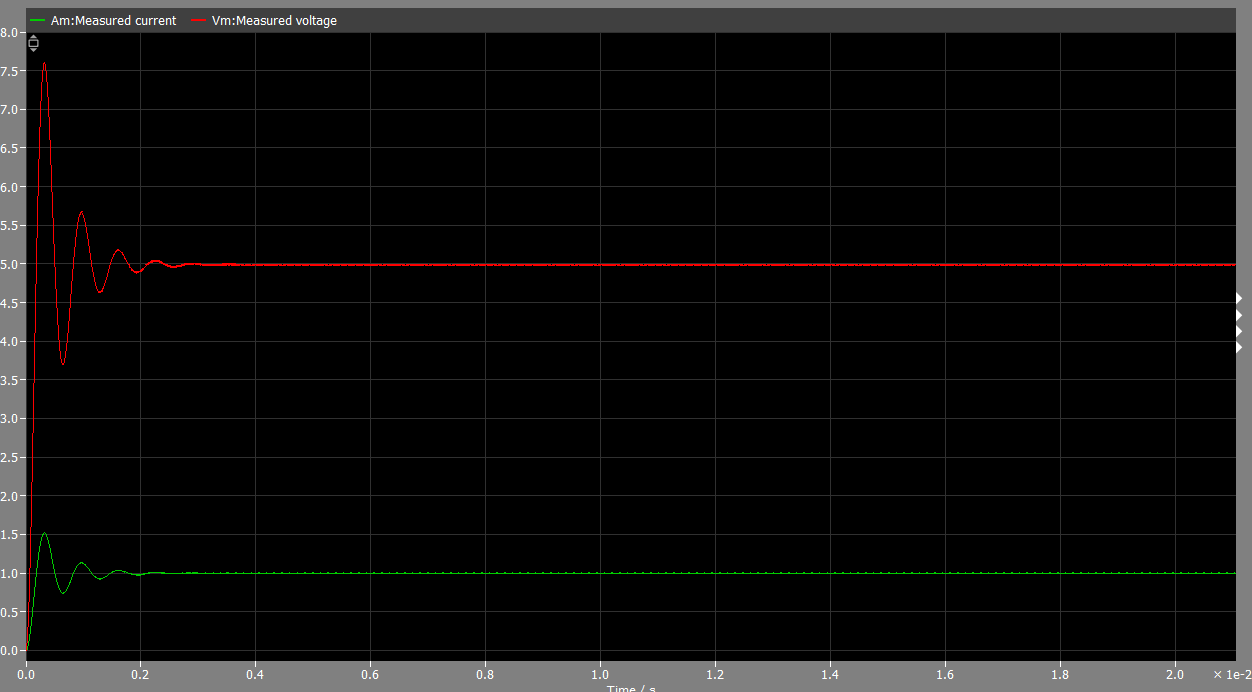
\includegraphics[width=\textwidth]{img/v_i_zoomed_constant_load.png}
        \caption{Startup behaviour of the uncontrolled converter}
        \label{fig:v_i_startup_uncontrolled}
    \end{subfigure}
    \hfill
    \begin{subfigure}[b]{0.49\textwidth}
        \centering
        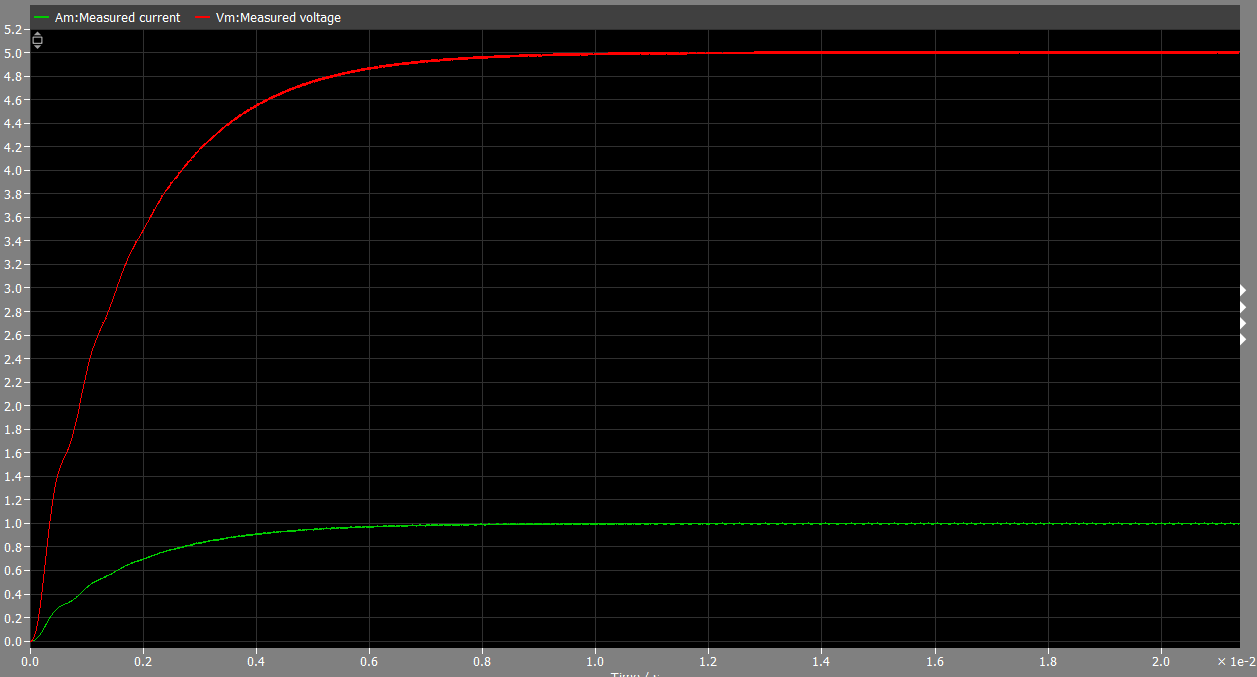
\includegraphics[width=\textwidth]{img/v_i_zoomed_control_constant_load.png}
        \caption{Startup behaviour of the controlled converter}
        \label{fig:v_i_startup_controlled}
    \end{subfigure}
    \caption{Comparison of the startup behaviour of the uncontrolled and controlled converter with current (green) and voltage (red) signals}
    \label{fig:comparison_startup}
\end{figure}

\begin{figure}[htbp]
    \centering
    \begin{subfigure}[b]{0.49\textwidth}
        \centering
        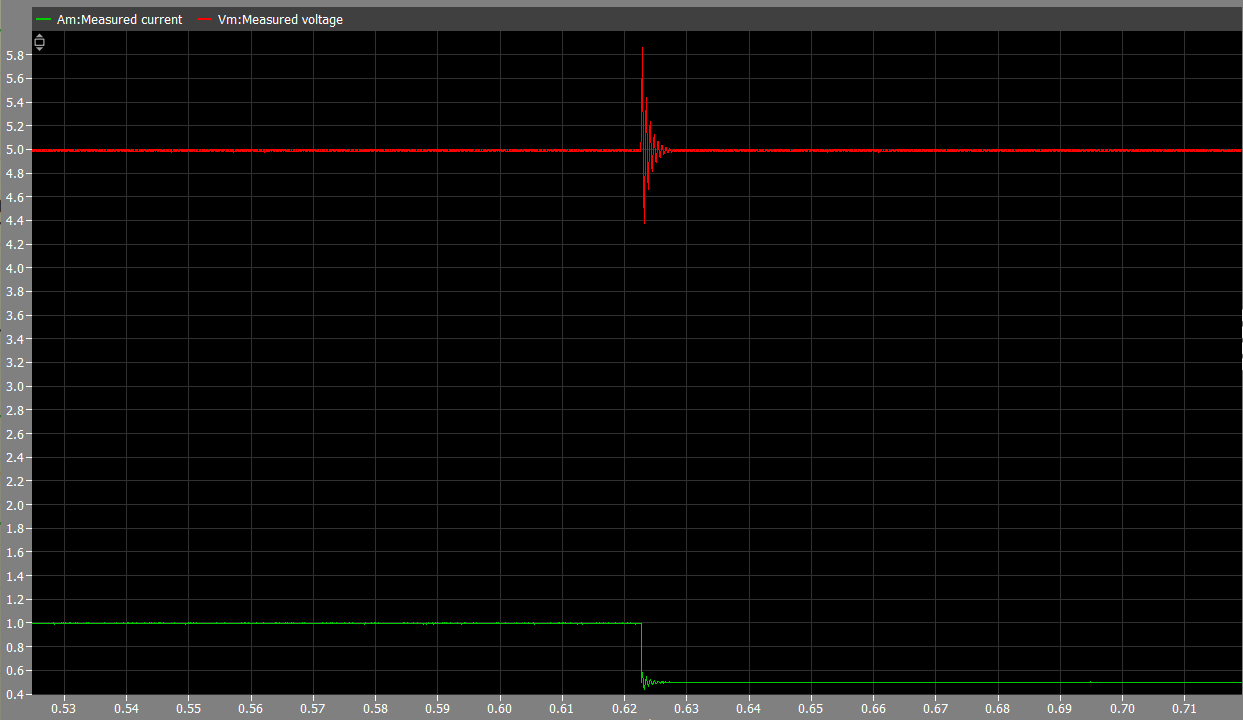
\includegraphics[width=\textwidth]{img/v_i_load_jump.png}
        \caption{load-jump behaviour of the uncontrolled converter}
        \label{fig:v_i_load_jump_uncontrolled}
    \end{subfigure}
    \hfill
    \begin{subfigure}[b]{0.49\textwidth}
        \centering
        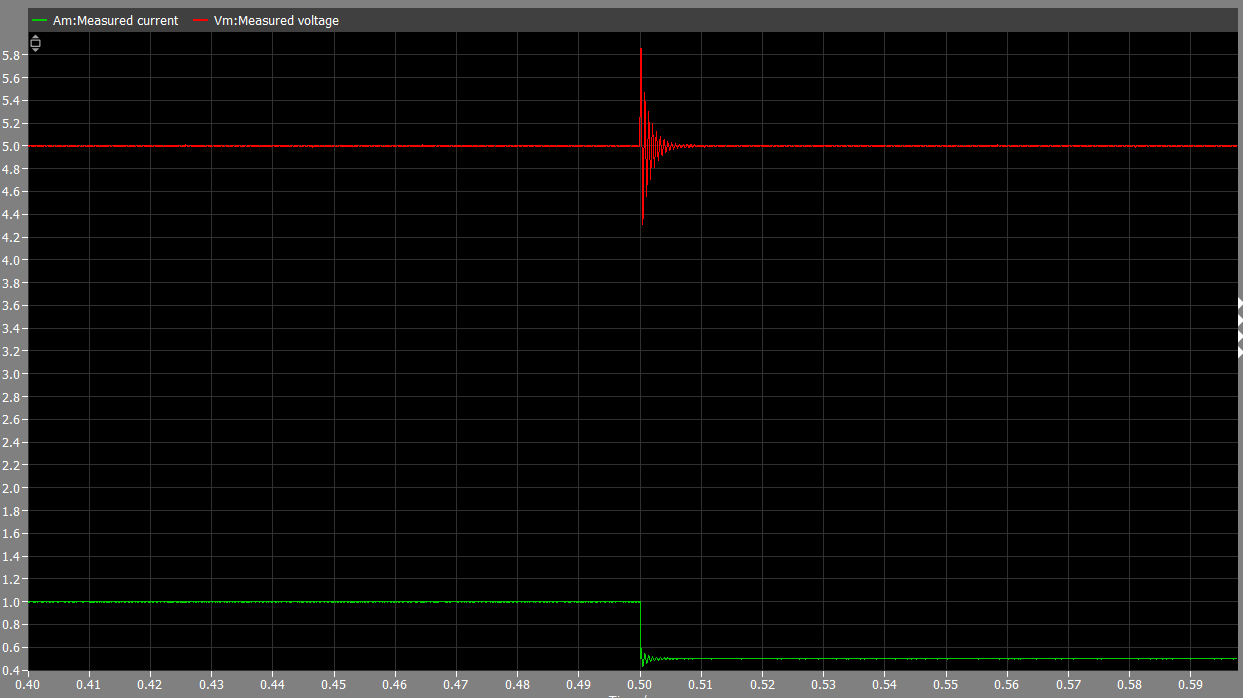
\includegraphics[width=\textwidth]{img/v_i_control_load_jump.png}
        \caption{load-jump behaviour of the controlled converter}
        \label{fig:v_i_load_jump_controlled}
    \end{subfigure}
    \caption{Comparison of the load-jump behaviour of the uncontrolled and controlled converter with current (green) and voltage (red) signals}
    \label{fig:comparison_load_jump}
\end{figure}

\begin{figure}[htbp]
    \centering
    \begin{subfigure}[b]{0.49\textwidth}
        \centering
        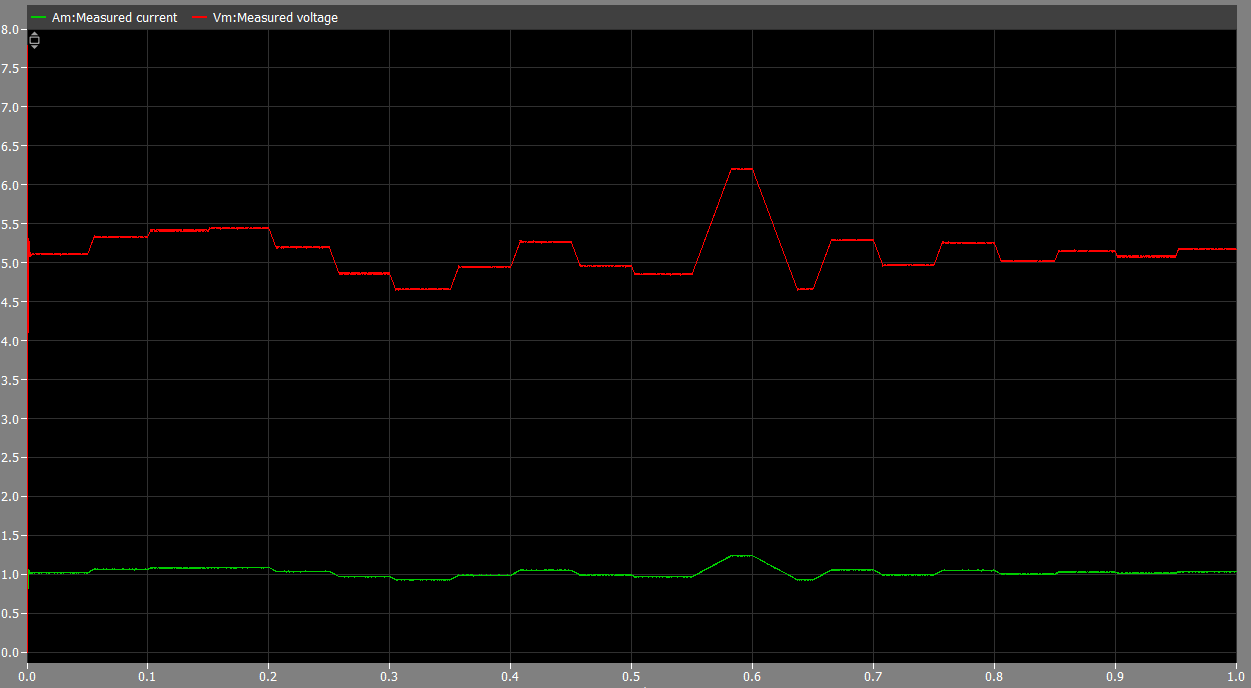
\includegraphics[width=\textwidth]{img/v_i_noise_constant_load.png}
        \caption{input noise feedthrough of the uncontrolled converter}
        \label{fig:v_i_noise_feedthrough_uncontrolled}
    \end{subfigure}
    \hfill
    \begin{subfigure}[b]{0.49\textwidth}
        \centering
        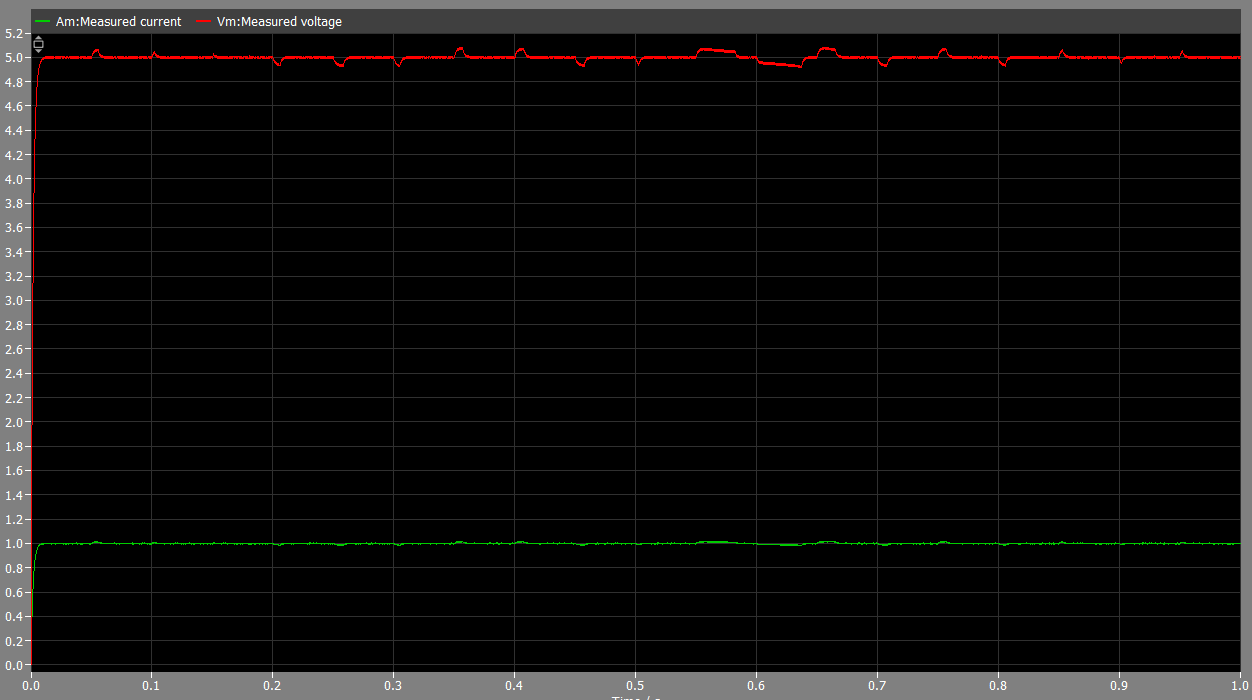
\includegraphics[width=\textwidth]{img/v_i_noise_control_constant_load.png}
        \caption{input noise feedthrough of the controlled converter}
        \label{fig:v_i_noise_feedthrough_controlled}
    \end{subfigure}
    \caption{Comparison of the input noise feedthrough behaviour of the uncontrolled and controlled converter with current (green) and voltage (red) signals}
    \label{fig:comparison_input_noise_feedthrough}
\end{figure}

\section{HIL Results}
\label{section:hil_results}

\begin{figure}[htbp]
    \centering
    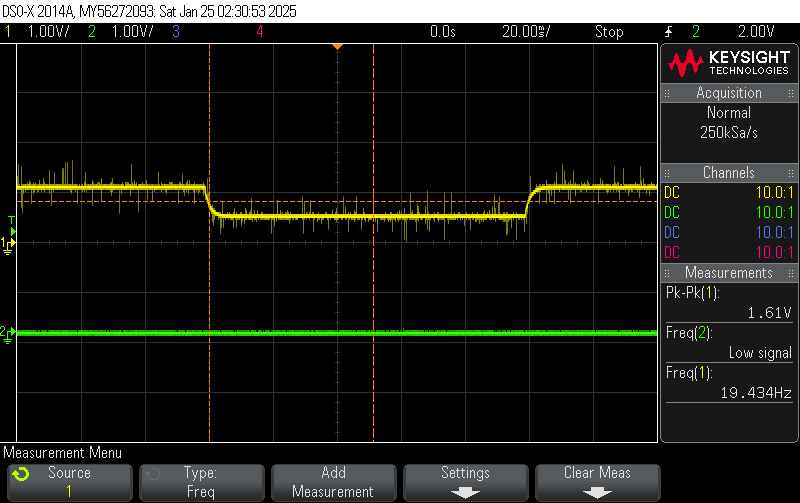
\includegraphics[width= 0.8\textwidth]{scope/scope_0.png}
    \caption{$V_{out}/5$ (ch1 - yellow) and PWM signal (ch2 - green) with vout }
    \label{fig:scope_output}
\end{figure}

\begin{figure}[htbp]
    \centering
    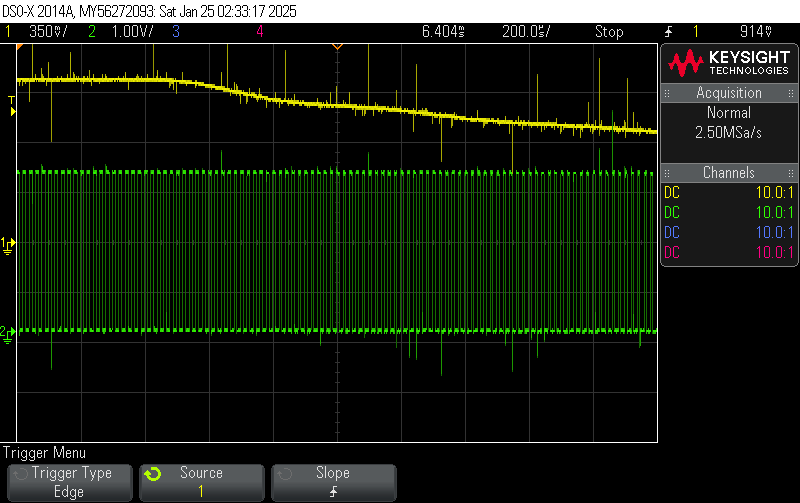
\includegraphics[width= 0.8\textwidth]{scope/scope_1.png}
    \caption{Scope output of the HIL simulation}
    \label{fig:scope_output}
\end{figure}



% EOF
    % !TEX TS-program = pdflatex
% !TEX encoding = UTF-8 Unicode
% !TEX root = ../main.tex
% !TEX spellcheck = en-US
% ****************************************************************************************
% File: discussion.tex
% Author: Jakob Spindler
% Date: 2024-10-16
% ****************************************************************************************
\chapter{Discussion}
\label{chapter:discussion}
The uncontrolled converter shows a significant overshoot and oscillation before settling to the working point at startup. The controlled converter shows a much smoother startup behaviour, but the settling time is longer than for the uncontrolled converter as shown in \autoref{fig:comparison_startup}.

The load-jump behaviour of the controlled converter still shows a spike at the load-jump, but quickly settles to the working point as can be seen in \autoref{fig:comparison_load_jump}, whereas the uncontrolled converter delivers a higher unwanted constant ouput voltage after the jump.

The input noise feedthrough of the controlled converter is significantly reduced, although not completely eliminated, compared to the uncontrolled converter as can be seen in \autoref{fig:comparison_input_noise_feedthrough}.

Overall, the behavioural characteristics of the converter have improved with the addition of the \Gls{acr:pid}-Controller.

% EOF

	\pagenumbering{Roman}
	\setcounter{page}{\value{romanpagecount}}
	\stepcounter{page}
	\printbibliography[heading=bibintoc] % This will add the bibliography to the table of contents
    
	%\addcontentsline{toc}{chapter}{\bibname}
	\listoffigures
	\addcontentsline{toc}{chapter}{\listfigurename}
	\listoftables
	\addcontentsline{toc}{chapter}{\listtablename}
	
 
	\clearpage
	\printglossary[type=\acronymtype] % input files created by makeindex
	\printglossary[type=symbolslist,style=symbolsliststyle] % input files created by makeindex

	% \appendix
	% % !TEX TS-program = pdflatex
% !TEX encoding = UTF-8 Unicode
% !TEX root = ../main.tex
% !TEX spellcheck = en-US
% ****************************************************************************************
% File: appendix.tex
% Author: Jakob Spindler
% Date: 2024-10-16
% ****************************************************************************************
\chapter{Appendix}
\label{chapter:Appendix}



\end{document}
% EOF